\label{chap:pdp_protocol}

This chapter discusses the underlying communication details of the packetized display protocol (PDP) architecture. First, it gives an overview of the protocol design methodology. Followed by a discussion of the generalized packet format. Finally, it discusses individual packet types. The central purpose of this chapter is to provide the reader with an understanding of the reasoning behind design decisions, as well as, to provide a detailed specification of the protocol.

\section{Design Methodology}
    The design methodology for the PDP protocol began with a number of critical design goals. The first goal was to design a scalable display system that was distributable and hardware agnostic. The second design goal was to provide a protocol that was relatively simple to implement without unnecessary complexity to ease the encoding and decoding process. A low overhead and fast decode process is crucial to ensuring latency is sub-frame\footnote{This refers to latency of that below the time it would take to buffer an entire frame. Which is a common synchronization method utilized in projector systems.} across the system. Additionally, simplifying these processes also eases potential hardware implementation mistakes, as well as, inefficiencies that could lead to reduced performance. The third goal was to provide dynamic intra-frame variable refresh rate (VRR) to enable better bandwidth utilization. In particular, to allow for regions of a display to be intelligently updated at different rates depending differences in input data. The fourth goal was to provide a path to utilize classical display protocol streams such as HDMI with PDP without introducing overhead. This is to allow for interoperability where necessary when utilizing classical display sources, and to ease migration to a PDP based system.

    \subsection{Comparison to Classical Display Protocols}
        In order to better understand how to design PDP, the constraints of classical display protocols were investigated to discern which features within these protocols conflict with the design goals of PDP. In addition, it was necessary to investigate whether these could provide a path forward in the design and development of PDP. Many versions of these protocols (DVI\cite{DDWG1999}, HDMI\cite{HDMIForum2018}, DisplayPort\cite{VESA2016}, etc.) provide similar feature-sets to end-users with the major focus being on increasing refresh rates and resolutions with each new specification. However, as discussed in Chapter~\ref{sec:classical_display_protocols}, their basis is rooted in the classical analog video specifications that utilize scan lines\cite{Neal1998}. This means, that signal timing utilizes vertical and horizontal blanking periods that consist of a front-porch, sync pulse, and back-porch; in addition to, the active video data to be displayed.

        For early analog display devices, these signals enabled operators to manually adjust horizontal and vertical hold times relative to the sync pulses in order to correct for the imprecise timing of early display hardware; but provide little benefit on modern hardware other than as an embedded method to support sending frames at a static interval, and to enable tearless buffer swapping in either double buffering\cite{FriedbergEtAl1990} or triple buffering schemes\cite{3dfx1997} utilized within GPUs\footnote{This is performed by swapping buffers during the vertical sync (vsync) interval of a frame\cite{3dfx1999,3dfx1999_2}. See Chapter~\ref{chap:display_protocols} for details about the vsync interval.}. In digital display technology, this represents an anachronism that impedes the goal of maximizing bandwidth utilization when driving a display by requiring the transmission of unnecessary data over the digital protocol. For example, a commonly utilized 1920 by 1080 pixel mode operating at \mbox{60 Hz}\cite{MythTVWebsite} on a modern display has a 16 percent blanking period overhead due to the specification of vertical and horizontal sync periods. Other examples can be seen in Table~\ref{tbl:modeline_overhead}.

        \begin{table}
            \centering
            \large
            \begin{tcolorbox}[tabularx={Y|Y|Y|Y|Y},title=\textbf{Modeline Overhead},boxrule=0.5pt]
            \textbf{Resolution} & \textbf{Refresh Rate (Hz)} & \textbf{Visible Pixels} & \textbf{Total Pixels} & \textbf{Overhead} \\ \hline
                \textbf{1920x1080} & \textbf{60}   & 2073600 & 2475000 & 16.2\% \\ \hline
                \textbf{1600x1200} & \textbf{60}   & 1920000 & 2700000 & 28.9\% \\ \hline
                \textbf{1280x1024} & \textbf{60}   & 1310720 & 1799408 & 27.2\% \\ \hline
                \textbf{1280x960}  & \textbf{60}   & 1228800 & 1800000 & 31.7\% \\ \hline
                \textbf{1280x800}  & \textbf{60}   & 1024000 & 1391040 & 26.4\% \\ \hline
                \textbf{1024x768}  & \textbf{60}   & 786432  & 1083264 & 27.4\% \\ \hline
                \textbf{500x500}   & \textbf{500}  & 250000  & 296100  & 15.6\% \\ \hline
                \textbf{500x500}   & \textbf{400}  & 250000  & 296100  & 15.6\% \\ \hline
                \textbf{500x500}   & \textbf{300}  & 250000  & 357500  & 30.1\% \\ \hline
                \textbf{500x500}   & \textbf{100}  & 250000  & 357500  & 30.1\% \\ \hline
                \textbf{500x500}   & \textbf{60}   & 250000  & 357500  & 30.1\% \\ \hline
                \textbf{500x500}   & \textbf{50}   & 250000  & 364000  & 31.3\% \\ \hline
                \textbf{500x500}   & \textbf{30}   & 250000  & 520000  & 51.9\% \\ \hline
                \textbf{500x500}   & \textbf{30}   & 250000  & 520000  & 51.9\% \\ \hline
                \textbf{500x256}   & \textbf{1000} & 131072  & 149460  & 12.3\% \\ \hline
                \textbf{500x256}   & \textbf{500}  & 131072  & 256000  & 48.8\% \\ \hline
                \textbf{500x256}   & \textbf{200}  & 131072  & 320000  & 51.9\% \\ \hline
                \textbf{500x256}   & \textbf{100}  & 131072  & 320000  & 59.0\% \\ \hline
                \textbf{500x256}   & \textbf{60}   & 131072  & 320000  & 59.0\% \\ \hline
            \end{tcolorbox}
            \caption[Modeline Overhead]{Modeline overhead for various resolutions and refresh rates\cite{MythTVWebsite}. Computed using active pixel area over total pixel area. 500x500 and 512x256 are typical modeline resolutions used on IRLED arrays.}
            \label{tbl:modeline_overhead}
        \end{table}

        These protocols also internally utilize a mode based display of data that requires the specification of the absolute width and height of display, as well as, a pixel clock which when used in conjunction with the vertical blanking information provides a total refresh rate as described in Chapter~\ref{sec:classical_display_protocols}. This means that the bandwidth requirements for a given mode are inherently static across all frames. In addition, this constrains the refresh rate for a display to be static in terms of both the intra-frame regions of the display and between frames. Effectively increasing the burden of synchronization, and impeding the introduction of dynamism into the display process. In recent years, work has been done to implement a limited form of variable refresh rate (VRR) display between frames for use with newer protocols\cite{AMDFreesync,NVIDIAGsync}. In essence, it allows for entire frames to be sent for display immediately once the rendering process has completed. The downside is that this generally requires specialized hardware support out of the scope of protocol specifications\footnote{A recent update of the HDMI 2.1 specification\cite{HDMIForum2018} seeks to integrate speed-limited form of VRR directly into the specification}, and requires entire full frames of data at the specified resolution.

    \subsection{A Path Forward with PDP}
        Internally PDP has no notion of blanking periods or porches for providing synchronization, and therefore does not encapsulate the inefficiencies inherent in the aforementioned protocols. Instead synchronization is controlled by the source through timing when data is sent. This means the high overheads as shown in Table~\ref{tbl:modeline_overhead} can be mitigated. Furthermore, because PDP allows for control over individual segments a large amount of bandwidth can be saved by updating parts of a frame at slower frame rates than other sections of a frame. Equation~\eqref{eq:bandwidth_saved} shows computing the savings where $p$ is the proportion of pixels operating at a slow frame rate, $r_f$ is the fast frame rate, $r_s$ is the slow frame rate, and $b_s$ the percentage of bandwidth saved.

        \begin{equation}
            b_s=1-\frac{(1-p)\cdot r_f + p\cdot r_s}{r_f}
            \label{eq:bandwidth_saved}
        \end{equation}

        %FIXME: double table and not referenced here
        \begin{table}
            \centering
            \large
            \begin{tcolorbox}[tabularx={Y|Y|Y|Y|Y},title=\textbf{Modeline Overhead},boxrule=0.5pt]
            \textbf{Slow Refresh Rate (Hz)} & \textbf{Fast Refresh Rate (Hz)} & \textbf{Visible Pixels} & \textbf{Total Pixels} & \textbf{Overhead} \\ \hline
                \textbf{1920x1080} & \textbf{60}   & 2073600 & 2475000 & 16.2\% \\ \hline
                \textbf{1600x1200} & \textbf{60}   & 1920000 & 2700000 & 28.9\% \\ \hline
                \textbf{1280x1024} & \textbf{60}   & 1310720 & 1799408 & 27.2\% \\ \hline
                \textbf{1280x960}  & \textbf{60}   & 1228800 & 1800000 & 31.7\% \\ \hline
                \textbf{1280x800}  & \textbf{60}   & 1024000 & 1391040 & 26.4\% \\ \hline
                \textbf{1024x768}  & \textbf{60}   & 786432  & 1083264 & 27.4\% \\ \hline
                \textbf{500x500}   & \textbf{500}  & 250000  & 296100  & 15.6\% \\ \hline
                \textbf{500x500}   & \textbf{400}  & 250000  & 296100  & 15.6\% \\ \hline
                \textbf{500x500}   & \textbf{300}  & 250000  & 357500  & 30.1\% \\ \hline
                \textbf{500x500}   & \textbf{100}  & 250000  & 357500  & 30.1\% \\ \hline
                \textbf{500x500}   & \textbf{60}   & 250000  & 357500  & 30.1\% \\ \hline
                \textbf{500x500}   & \textbf{50}   & 250000  & 364000  & 31.3\% \\ \hline
                \textbf{500x500}   & \textbf{30}   & 250000  & 520000  & 51.9\% \\ \hline
                \textbf{500x500}   & \textbf{30}   & 250000  & 520000  & 51.9\% \\ \hline
                \textbf{500x256}   & \textbf{1000} & 131072  & 149460  & 12.3\% \\ \hline
                \textbf{500x256}   & \textbf{500}  & 131072  & 256000  & 48.8\% \\ \hline
                \textbf{500x256}   & \textbf{200}  & 131072  & 320000  & 51.9\% \\ \hline
                \textbf{500x256}   & \textbf{100}  & 131072  & 320000  & 59.0\% \\ \hline
                \textbf{500x256}   & \textbf{60}   & 131072  & 320000  & 59.0\% \\ \hline
            \end{tcolorbox}
            \caption[Modeline Overhead]{Modeline overhead for various resolutions and refresh rates\cite{MythTVWebsite}. Computed using active pixel area over total pixel area. 500x500 and 512x256 are typical modeline resolutions used on IRLED arrays.}
            \label{tbl:pdp_efficiency}
        \end{table}


        %FIXME: Add figure that shows better bandwidth utilization of PDP?
        %FIXME: Relate back to the design goals of PDP


\section{Packet Format}
    %FIXME: REAL PROPOSAL slides 31 and 32 talk about packet considerations and details
    %FIXME: insert packet format from REAL PROPOSAL slide 34 and 36

\section{Packet Types}

    Figure~\ref{fig:packets} shows the basic packets used for communication within PDP. These are strictly for data transfer and synchronization of system operations, and do not include other aspects such as system setup or enumeration\footnote{System setup and enumeration are typically system specific operations and outside of the current PDP Design, but may be incorporated in the future}. These packets are organized into type specific fields of some set word-size. The exact size of word fields is left abstracted to allow for an optimal implementation to be used in practice. For example, a system may utilize 24-bit word size if an array has a native 24-bit pixel size, or 32-bit word size if the hardware transport layer has a specific optimal word size. Typically, a multiple of 8-bit word size would be utilized in practice, as most hardware architectures (such as x86) utilize some multiple of this size. In any given implementation, the word size of all fields must match, in order to simplify decoding operations. This allows for fixed-size decoding of incoming data, which simplifies processing and firmware implementation, as well as, can ease timing constraints and enforce non-variability in the decoding time of incoming packets of data. In general, PDP packets are designed to send a minimal amount of header data to lower overhead and ordered in a way to minimize buffering requirements to enable real-time processing.

    \begin{figure}
        \centering
        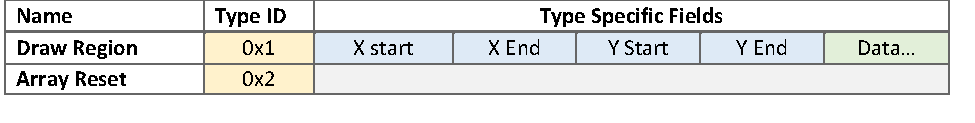
\includegraphics[width=1.0\textwidth]{fig/packet_chart.pdf}
        \caption{List of PDP Packets}
        \label{fig:packets}
    \end{figure}

    In terms of the protocol itself, PDP uses a single global coordinate system to refer to pixel locations on a display array. For example, a 512 by 512 pixel array would have coordinates from 0 to 511 in both the horizontal and vertical directions. All packets referencing sub-regions of this display would utilize coordinates that map to some rectangular sub-region of the display. Any overlapping regions of data would be composited during system operation with priority given to data segments sent at higher frame rates.

    PDP Packets are segmented into three types, a draw region packet, array reset packet, and trigger packet. All packets consist of a Type ID field of word-size. The draw region packet is used to send a rectangular sub-region of pixel data in global array coordinates. It has fields for the start and stop horizontal and vertical coordinates (defined inclusively) followed by individual pixel data. For example, suppose a scene generator were to send a packet of data from array region 10 to 19 along the X axis and 20 to 29 along the Y axis, a total of 100 pixels of data would follow the packet coordinates given that the packet specifies a 100 pixel sized region.

    The second packet, array reset, is utilized to indicate that quadrants on a given array should be cleared. It consists of an array specific quadrant bit-mask used to indicate which quadrant to reset. Any unused bits are reserved. This type of packet would be utilized exclusively between compositor and array tile links.

    The third packet, trigger, is used to implement a trigger based synchronization within in PDP. It consists of a system specific action bit-mask used to indicate the type of operation to trigger. In IRLED array systems, the coordinator of synchronization is dependent on the array itself and the different components within the system. In some systems, a sensor may be used as the source of synchronization, in other systems, another component may be utilized. Other aspects of system operation may even be triggered outside of the system synchronization interval based off of other events. For the reason, PDP has opted for a trigger based approach to synchronization. This approach allows for synchronization, data transfer, and computation to be custom tailored to an individual systems use-case. For example, the action mask could be used to trigger the generation of the next frame to be displayed when needed, the source of which is defined by the system itself. Another example would be utilize the action mask to indicate that further computations (such as scene generation) stall until otherwise indicated.

\section{PDP Frames}
    %FIXME: insert picture from slide 38 of real proposal
